\documentclass[11pt]{article}   % Mandatory
\usepackage[T1]{fontenc}        % Support for fonts with æøå and other foreign characters.
\usepackage[utf8]{inputenc}     % Support for UTF-8 encoded input documents
\usepackage{fullpage}
\usepackage{graphicx}           % Support for including graphics as png, gif, and jpeg
\usepackage{amssymb}            % Support for alterantive symbols
\usepackage{amsmath}            % Support for mathematical symbols
\usepackage{listliketab}        % Support for tabulated lists
\usepackage{enumitem}           % Support for indented description items and more
\usepackage[parfill]{parskip}   % Support for American style paragraphs
\usepackage{color}              % Support for colored text
\usepackage{listings}           % Support for code listings
\usepackage{nameref}            % Enables refernces to names.
\usepackage{makeidx}            % For creating indexes
\usepackage{wasysym}            % For symbols as \smiley
\usepackage{hyperref}    		% For using URLs
\usepackage{utilities/petri}    % For doing petrinet vector graphics
\newcommand{\epns}{\textbf{ePNS}}
\newcommand\writer[1]{\nobreak\begin{flushright}\small\textbf{Author: \large\textit{#1}}\end{flushright}}
\makeindex

\title{Handbook\\ \epns}
\author{Group E}
\date{Autumn 2012}

\begin{document}
\maketitle

\tableofcontents

\section{Introduction}
\label{sec:introduction}
\writer{Anders}

This is a handbook for the \index{ePNS}``group \textbf{e} \textbf{P}etri \textbf{N}et \textbf{S}imulator'': \epns.
The purpose of \epns{} is to facilitate \index{track based simulation}track based simulations of Petri nets.
A track based simulation is understood as a simulation of a world, where objects move along tracks,
following a set of rules given by the Petri net. The objects can be simulated as trains on tracks, cars on roads,
or any other object following a predefined route.

\subsection{What can be simulated?}

Petri nets are, with the addition of \index{inhibitor arc}inhibitor 
arcs\footnote{Inhibitor arcs prevents transitions from fireing unless the associated place is empty.
Inhibitor arcs are not implemented by \epns{} yet.},
Turing complete,
meaning that they can implement any computer program.
We will not formally prove this property, as it is out of scope for this
assignment.
But it is not hard to understand why: the inhibitor arc makes it possible to
implement a NAND gate (see figure \ref{fig:petri-nand}).
All binary operations can be expressed using the NAND operation, some examples:
\begin{align*}
    \overline{A} &= \overline{A \cdot A}               
	                & NAND(A, A) \\
    A \cdot B    &= \overline{\overline{A \cdot B}}
    				& NAND(NAND(A, B), NAND(A, B))\\
    A + B        &= \overline{\overline{A + B}} = \overline{\overline{A} \cdot \overline{B}} 
    				& NAND(NAND(A, A), NAND(B, B)) \\
    A \otimes B  &= A \cdot \overline{B} + B \cdot \overline{A}
    			  = \overline{\overline{A} \cdot \overline{B}} \cdot \overline{A \cdot B}
    				& \text{use previous formulas \ldots}
\end{align*}

\begin{figure}[htp]
\begin{center}
\begin{petri}
    \node at (0, 0) [inputplace] (inputA) {$A$};
    \node at (0, 3) [inputplace] (inputB) {$B$};
	\node at (2, 1.5) [transition] (andtransition) {$T_1$};
	\node at (4, 1.5) [place] (andoutput) {$A B$};
	\node at (6.5, 1.5) [inhibitor] (inhibitor) {};
	\node at (5.6, 1.8) {inhibitor};
	\node at (7, 1.5) [transition] (nandtransition) {$T_2$};
	\node at (9, 1.5) [place] (nandoutput) {$\overline{A B}$};
	\draw [->,arc] (inputA) to [out=60,in=200] (andtransition);
	\draw [->,arc] (inputB) to [out=-60,in=160] (andtransition);
	\draw [->,arc] (andtransition) to [out=0,in=180] (andoutput);
	\draw [->,arc] (andoutput) to [out=0,in=180] (inhibitor);
	\draw [->,arc] (nandtransition) to [out=0,in=180] (nandoutput);
	%\draw [->,arc] (connection) to [out=210,in=330] (track);
	%\draw [->,arc] (semaphore) -- (connection);
\end{petri}
\caption{Petri net for a NAND gate}
\label{fig:petri-nand}
\end{center}
\end{figure}

Consequently not all Petri nets are suited for track based simulations.
The main concept of Petri nets are that transitions consume tokens from places connected with inbound arcs,
and produces tokens in places connected with outbound arcs.

Therefore don't expect any Petri net to produce a logical or useful 3D
simulation. Not even if it doesn't include inhibitor arcs.

In \epns{}, if a token is produced in a place associated with a track,
the token itself will be associated with a moving object.
Therefore, Petri nets that produce the same amount of tokens as it consume
will be most suited for \epns{} simulations.
This is not a mandatory property, but it ensures that the moving objects don't disappear or
appear out of the blue\footnote{In a production line simulation it might be on purpose.
For example, four wheels and a car body disappears and a car arises.}.

Other places can be associated with objects that show the state of the underlying logic.
In the train simulation world, they could be traffic lights or switches.

However, other places should be designated to receive input from the user.
Such places might not be part of the initial logic, but should be added where input is needed.

\subsection{How to use the handbook?}

In the \nameref{sec:installation} section, the necessary steps to have a running
installation are reviewed. An installation includes the Eclipse IDE and additional modules. 

For first time users, the section \ref{sec:tutorial} (\nameref{sec:tutorial}) will cover 
the steps needed to create a simple Petri net simulation. These steps include:
\begin{itemize}
  \item Creating the Petri net.
  \item Laying out the tracks and the positions of input and output objects in the associated geometry model.
  \item Selecting the appearance of the elements.
  \item Creating the configuration for the simulation.
  \item Running the simulator.
\end{itemize}

For more experienced users, the section \ref{sec:userguide} (\nameref{sec:userguide}) will provide
detailed information on the various steps in creating more complex simulations. 

Please consult the index and glossary for information on specific subjects.

\subsection{Basic functionality of ePNS}
\writer{Cosmin}
In order to use \epns, the application user starts by using the \textbf{Petri net Editor} to create
and configure the Petri net and the \textbf{Animations} that are executed during the simulation.
These will be later loaded by the \textbf{Graphical Simulator}, which, after being started, will
simulate the movement of tokens through the Petri net and will execute the configured animations,
resulting a visual representation of the Petri net's simulation on the screen.

Then, using the \textbf{GeometryEditor}, the \textbf{Geometry} would be created. It would be later
used by the \textbf{Graphical Simulator} in order to know how (on which paths) to move objects/token
representations and where to place different objects in the 3D space\footnote{Even though the
geometry is specified in a 2D space, during the simulation, all the object representations will be
drawn as 3D objects moving on a plane.}.

The \textbf{Graphical Simulator} also requires information about the \textbf{Appearance}, in order
to know how to represent tokens, tracks and other objects during the simulation. It is a simple
editor that connects labels (keys) with 3D Models(vrml, png, jpg \ldots), textures or just plain
data (Colors, Shapes).
  
The last step is to create a \textbf{Configurator} that connects the previously created
configurations and allows the user to start the graphical simulation. When started, the
\textbf{Graphical Simulator} reads the state of the simulation from the \textit{Petri net}. This read
state does not include exact positions of tokens in space, this information being loaded from the
\textit{Geometry}, or appearance information, loaded from the \textit{Appearance}. After
initialization, the Graphical Simulator displays the state of the simulation and handles all the
users' interaction as specified in the rest of this document.

For further details of what exactly each of the components allows the users to do please check the
following section or, in order to get more details, regarding implementation of \epns, please read the
\textit{System Specification}.

\subsection{General concepts}
\writer{Cosmin}
\label{oa:generalconcepts}
This subsection will introduce the general concepts used in the \epns system. More details are
provided in the \textit{System Specification}, however the most important concepts are presented below.

First of all, the classical concepts of \textbf{Petri nets} have been extended to accommodate the
required information for the graphical visualization of the simulation:
\index{Petri net} 
\begin{description}
\index{Petri net!Input Place}
\item[Input Places] - in order to provide the users with more power and customizability, some of the
Places in the Petri net can be configured to allow users, during the graphical simulation, to drop
(create) tokens. These are called \textit{Input Places} and act as normal Places in all other
respects, except for that they permit the possibility of a token being created there. For example,
in a train track simmulation, it allows the creation of simulation features such as a Traffic lights
or switches with which the users can interact during the graphical simulation.
\index{animation}
\item[Animations] - can be associated by the user to a particular Place and are run when a Token is
added on that Place, either by result of executing a transition or by being dropped there (after a
user interaction). Even though the token is removed from the source Places of the fired Transition,
they are not available for firing a new Transition until the animations associated with a place are
finished. More details will be specified later, but the supported animation types include: moving an
object on a path, showing or hiding objects, wait a fixed amount of time.
\item[Place Appearance] - each Place can have an associated appearance, describing how it must look
like in the Graphical Simulator.
\item[Token Appearance] - each Token can have an associated appearance, describing how it must look
like in the Graphical Simulator. Thus, the appearance of a Token will not change based on a place.
This will allow multiple tokens, with different representations, to be on the same place/track.
\item[Arc Identities] - each arc can have attached an identity used to control the flow of tokens
(or, more precisely, of token representations) in the simulation. For e.g., if we have a Transition
with one input Arc and two output Arcs and we take the case of simulating a train running on a
track, using the same identity on the input Arc and on one of the ouput Arcs will tell the Graphical
Simulator to move the Token representation (a train), which came on the input Arc, on the
corresponding output Arc. This allows a token representation to move continously in the direction
the user wants, without being destroyed or unnecessarily recreated.
\end{description}

Regarding the \textbf{Geometry}, as defined, it allow the users to specify the positions of objects
and the paths on which they move in the simulation space. The most important related concepts that
need to be presented at this point are:
\index{geometry}
\begin{description}
\index{Petri net!Track}
\item[Track] - defines how a curve (or line), on which an animation can take place, looks like. It
can also be connected with information about what the surface of this track looks like and usually
are used as graphical representations of Places.
\index{Petri net!Simple Position}
\item[Simple Position] - defines just a position in the simulation space and can be connected to the
an appearance it has. Can be used for completing the specification of some animations, for
representing an Input Place or just for displaying simple objects during the simulation.
\end{description}

Referring to the \textbf{Appearance}, it allow the users to easily define how objects look like
during the simulation. In \epns, there are mainly two big types of appearances that can be
configured:
\index{appearance}
\begin{description}
\item[Shape] - defines how a 3D Object displayed in the simulation should look like. For example, it
can be a reference to a file storing a 3D Model, which can then be loaded in the application or it
can simply be a 3D Object, such as a Cube or Sphere.
\item[Surface] - defines how a surface displayed in the simulation should look like. It can be
applied, for example, to a train track, and it could be either just a Color or a reference to a file
containing a texture that can be applied on the surface.
\end{description}



\section{Installation}
\writer{Cosmin}
\label{sec:installation}

This section discusses the installation of the product and presents the requirements and main steps
necessary to make the system work.

\subsection{Prerequisites}
Our product is built as a series of extensions for the Eclipse Development Platform and requires
Java. Furthermore, ePNK 0.9.4 has to be set up in Eclipse and the Java3D 1.5.1 library has to be
installed.

First of all, \textit{Eclipse 4.2.0} (Juno) has to be installed on the computer. The installation
can be done by following the instructions found in the Eclipse Install Guide
\footnote{http://wiki.eclipse.org/Eclipse/Installation} or by navigating to
\url{http://www.eclipse.org/downloads}.

Secondly, \textit{Java Runtime Environment 1.6} has to be installed. Setting up the Java
environment can be done by following the instructions found on the Java homepage,
\url{http://www.java.com} or by navigating directly to the Java Downloads page
\footnote{http://java.com/en/download/manual.jsp}.

The \textit{ePNK} can be installed, as an Eclipse extension, by following the details provided on
its homepage, \url{http://www2.imm.dtu.dk/~eki/projects/ePNK/install-details.html}. For more
details, ePNK's manual \footnote{http://orbit.dtu.dk/getResource?recordId=275136} can also be
consulted.

The last requirement, \textit{Java3D} library, can be set up by following the instructions on the
product's home page, \url{http://java3d.java.net/} or on the install guide page
\footnote{http://download.java.net/media/java3d/builds/release/1.5.1/README-download.html}.

\subsection{Product installation}
As mentioned before, the product has to be installed as an Eclipse plugin. The final version of
the product will be available as an Eclipse plugin that can be installed via an update 
site (or, for offline installation, as a site of files that need to be copied in the Eclipse plugins 
directory). The plugin will be available only after Eclipse has been restarted, if it was running.

During the development period, the product is available as a set of projects\footnote{The latest
version is available at https://svn.imm.dtu.dk/se2/svn/e12-groupE/project/} that have to be
downloaded locally and imported into the Eclipse Development Environment. After opening the projects, a
Runtime Eclipse Workbench has to be started by selecting one of the projects and then by clicking on
the \textit{Run} command.

\section{Tutorial}
\label{sec:tutorial}
\writer{María}

This section is a practical guide that will show you the basic functionality of the ePNS Petri net simulation system;
the tutorial will go through a simple example to allow you to learn how to use it.

Imagine that you want to simulate a scenario in which a red cube follows a circular line when you press a button. 
First, you need to model the corresponding Petri net where places are visually represented by an image in a 
2D plane \index{2D plane} (in this case, the line and the button), and tokens can represent 3D objects 
\index{3D object} moving on top of the 2D image (in this case, the cube following the line). Transitions have no 
visual representation, but they are of course still necessary for the proper performance of the Petri net. 
The model designed for this scenario could be the one shown in Figure \ref{fig:basic_pn}.

\begin{figure}[htp]
    \begin{center}
    \begin{petri}
        \node at (0, 0) [place] (track) {};
        \node at (3, 2) [inputplace] (semaphore) {};
        \node at (3, 0) [transition] (connection) {};
        \node at (0, 0) [token] {};
        \draw [->,arc] (track) to [out=30,in=150] (connection);
        \draw [->,arc] (connection) to [out=210,in=330] (track);
        \draw [->,arc] (semaphore) -- (connection);
        \draw [-,arc] (2.8, 2.2) -- (3.2, 1.8);
        \draw [-,arc] (2.8, 1.8) -- (3.2, 2.2);
    \end{petri}
    \caption{Petri net model}
    \label{fig:basic_pn}
    \end{center}
\end{figure}

The place on the left is the one that will represent the circular line, and the one with the dashed line 
will represent the button. Note that this second place is not an ordinary place: it is an \textit{input place} 
\index{input place}, where tokens can be externally inserted during the simulation. When the button is clicked, a 
token will appear in that input place, and the transition will be fired. In an ordinary Petri net, when this happens
the tokens in the transition's source places are removed from said places and new ones appear in the transition's target 
places. However, \epns{} offers the posibility of putting identities to arcs to prevent tokens from being destroyed in the 
process and preserve its appearance (if it's a cube, a train, a car...) during the simulation. \index{ePNS Petri net!attributes!identity}

The model can be created using the Petri net editor \index{editors!Petri net} with \epns's custom Petri net type (ePNS Petri net) 
\index{ePNS Petri net}. For this purpose, you have to create a PNML document and edit it, creating the places, transitions 
and tokens, set their attributes and conect them accordingly with the help of arcs. To do this, you must follow these steps:

\begin{enumerate}
  \item In the runtime workbench, click "File > New > Project > General > Project". Click on "Next", give it a 
  name and click "Finish".
  \item Right click on the created project, select "New > Other > ePNK > PNML Document" and click "Next" \index{PNML Document}.
  \item The project folder should already be the parent folder. If not, change it to make it so. Give a name to 
  your new file and click on "Finish" (note that you should keep the \textit{.pnml} extension.
  \item Open the file and you will see a tree editor. Expand the root node and right click on "Petri Net Doc". 
  Add a Petri net by selecting "New Child > Petri net (ePNS Petri net)" (See Figure \ref{fig:tut01}).
  \item In the newly created Petri net, right click and select "New Child > Page" (See Figure \ref{fig:tut02}).
  \item Double click on the created Page to open the graphical editor.
  \item In this editor, you can add Nodes (Places and Transitions) by clicking on the corresponding symbol in the 
  \textit{Palette} on the right hand side of the screen, and clicking on the canvas to place it. (See Figure \ref{fig:tut03}).
  \item You may connect Nodes with the Arc tool in the Palette. To do this, select the Arc icon, click on the desired 
  source Node and drag on top of the desired target Node.
  \item To modify the attributes of an element, right click on it and click on "Show Properties View". \index{Properties View} 
  The selected element's properties can be changed in this view.
  \item Every element has an attribute called "Id". Change it to be able to differentiate each component. For example, 
  assign "P1" to the classical Place, "P2" to the Input Place, "T1" to the Transition, "A1" to the Arc connecting the Input Place 
  with the Transition and "A2" and "A3" to the other two Arcs.
  \item Places have an attribute that indicates if they are Input Places. Edit it in each Place to give it the correct 
  value (true or false). \index{ePNS Petri net!attributes!Interactive Input} 
  \item The aforementioned Identity attribute of Arcs can be changed in the Properties View. Set the identity of "A2" and "A3" to 1. You will 
  see that the color of the Arc changes according to its Identity (in this case the arcs will turn red).
   \index{ePNS Petri net!attributes!identity} 
  \item When you have finished the structure, you must add the Token. To do this, select the Label tool from the Palette and 
  place a Label on the canvas. Use then the Link Label tool to attach the Label to the ordinary Place (in our case, Place P1) 
  and select "Token" (See Figure \ref{fig:tut04}).
\end{enumerate}

\begin{figure}[htp]
\begin{center}
  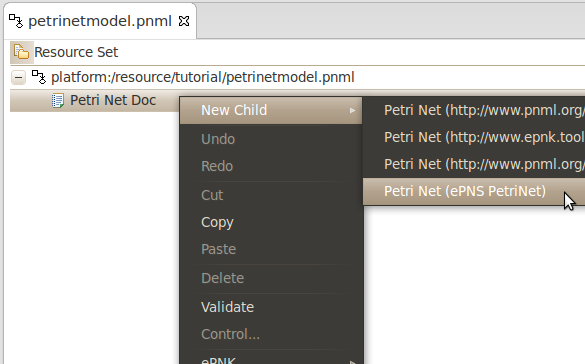
\includegraphics[width=10.0cm]{image/tutorial/Tutorial_01.png}
  \caption{Creation of the Petri net model}
  \label{fig:tut01}
\end{center}
\end{figure}

\begin{figure}[htp]
\begin{center}
  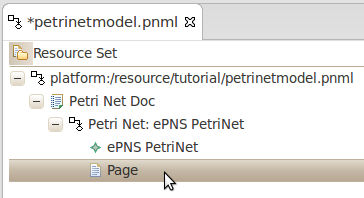
\includegraphics[width=6.0cm]{image/tutorial/Tutorial_02.png}
  \caption{PetriNet Page}
  \label{fig:tut02}
\end{center}
\end{figure}

\begin{figure}[htp]
\begin{center}
  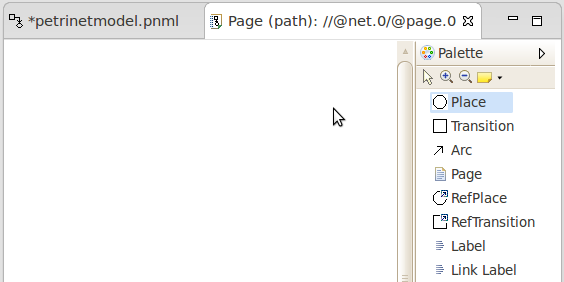
\includegraphics[width=10.0cm]{image/tutorial/Tutorial_03.png}
  \caption{Palette}
  \label{fig:tut03}
\end{center}
\end{figure}

\begin{figure}[htp]
\begin{center}
  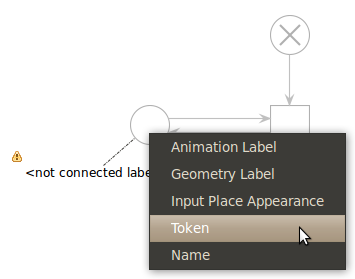
\includegraphics[width=8.0cm]{image/tutorial/Tutorial_04.png}
  \caption{Creation of tokens}
  \label{fig:tut04}
\end{center}
\end{figure}

\newpage 
You should now have a Petri net model similar to the one in Figure \ref{fig:tut05}.

\begin{figure}[htp]
\begin{center}
  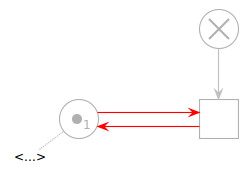
\includegraphics[width=5.0cm]{image/tutorial/Tutorial_05.png}
  \caption{PetriNet model}
  \label{fig:tut05}
\end{center}
\end{figure}

You can now proceed to the Geometry editor \index{editors!geometry}, where you will draw the 2D path along which the 
Token representations (the cube in this example) will move. The Geometry for this particular example will consist of a 
circular line and a separate point (where a button that represents the Input Place will appear in the final visualization
to allow the user to create a new Token in the Input Place to make the Transition fire). 

The following steps describe how to do this:
\begin{enumerate}
  \item Select the project you created before in the Project Explorer and right click on it to select "New > Other > 
  ePNS > Geometry Diagram". Click "Next".
  \item Once again, the project you created should be selected as the parent folder (if it is not, change it). Give 
  your Geometry Diagram a name (keeping the \textit{.geometry\_diagram} extension). Click "Next".
  \item The Geometry Model needs also to be created together with the Geometry Diagram. Select your project as the parent 
  folder and give your Geometry Model a name (keeping the \textit{.geometry} extension). Click "Finish".
  \item The file with the \textit{.geometry\_diagram} extension is the graphical editor. Open it to start building your Geometry.
  \item Create a Track Position on the canvas (in this example, this Track Position will represent the beginning and
  end of the same Track, the only one used, but it could be the beginning of a Track and the end of a different one;
  for more information see \ref{sec:userguide:geometry:elements}), select the Track tool and click on the Track
  Position you just created. A Track with the shape of a square will appear. You can click on the Track and modify
  its shape to create a circle.
  \item Give a name to the Track by filling the Label attached to it, for example "circle".
  \item To create the button that will allow the cube to move, you have to add a SimplePosition (for more information
  on SimplePosition objects, see \ref{sec:userguide:geometry:elements}) to the canvas. Give also a name to this
  element, for example "point".
\end{enumerate}

The Geometry model should now look like Figure \ref{fig:tut06}, where the empty square is the Track Position, the Track
symbol with the word "circle" is the Label and the square with the dashed line and the word "point" is the SimplePosition.

\begin{figure}[htp]
\begin{center}
  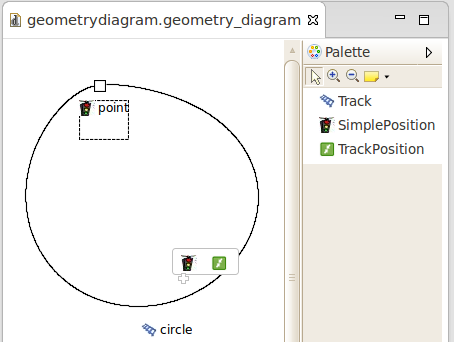
\includegraphics[width=10.0cm]{image/tutorial/Tutorial_06.png}
  \caption{Geometry model}
  \label{fig:tut06}
\end{center}
\end{figure}

Now that you have the Geometry model, you have to specify which Geometry object corresponds to each Place. For this purpose, 
you have to assign a Geometry Label \index{ePNS Petri net!attributes!Geometry Label} to each place of the Petri net model.
\begin{enumerate}
\item Go back to the Petri net graphical editor, create a Label and link it to a Place. You will see that you can set the Label 
to the type "Geometry Label" (See Figure \ref{fig:tut07}), where you must write the name of the correponding Geometry element.
\item Add a \textit{Geometry Label} to the ordinary Place and call it "circle" (See Figure \ref{fig:tut08}).
\item Also add a \textit{Geometry Label} to the Input Place and assign the name "point".
\end{enumerate}

\begin{figure}[htp]
\begin{center}
  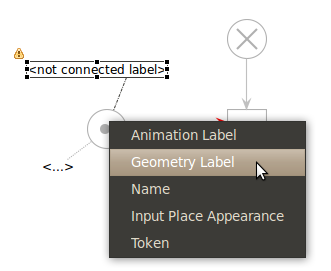
\includegraphics[width=7.0cm]{image/tutorial/Tutorial_07.png}
  \caption{Create Geometry Label}
  \label{fig:tut07}
\end{center}
\end{figure}

\begin{figure}[htp]
\begin{center}
  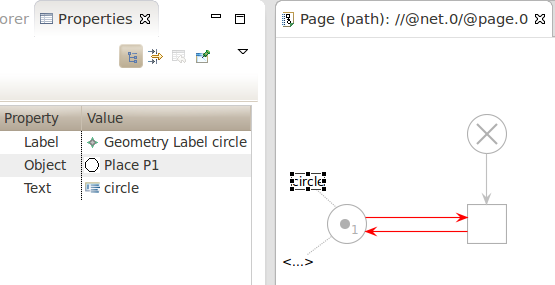
\includegraphics[width=10.0cm]{image/tutorial/Tutorial_08.png}
  \caption{Geometry Label of the ordinary place}
  \label{fig:tut08}
\end{center}
\end{figure}

\newpage
Now, you need to indicate the behaviour of the simulation: when you click on the button, a red cube shall move following the 
circular line at a certain speed. This is done by assigning an Animation \index{animations} to the ordinary Place.
\begin{enumerate} \index{ePNS Petri net!attributes!Animations}
  \item In the Petri net graphical editor, create a Label and connect it to the ordinary Place, selecting "Animation Label"
  (See Figure \ref{fig:tut09}).
  \item As the Label needs a correct Animation, a warning symbol will appear until you write it. To do that, edit the Label 
  and write "move(3.0)" on it. This is to specify that the cube shall move at a speed with the value 3, and it will move along 
  the Track named "circle" because that is the name of the previously created Geometry Label.
\end{enumerate}

\begin{figure}[htp]
\begin{center}
  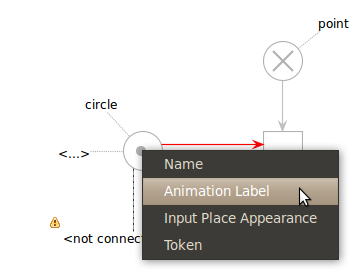
\includegraphics[width=7.0cm]{image/tutorial/Tutorial_09.png}
  \caption{Create Animation Label}
  \label{fig:tut09}
\end{center}
\end{figure}

The Simulator does not know yet how the different elements of the Petri net model should look like. In particular, the Appearance of the
Token (a red cube), the Input Place (a button) and the ordinary Place (a track) should be set. To do this, an Appearance configuration 
has to be created. \index{editors!appearance} \index{appearance}
\begin{enumerate}
  \item Select the project you created before in the Project Explorer and right click on it to select "New > Other > ePNS > 
  Appearance Model". Click "Next".
  \item Once again, the project you created should be selected as the parent folder (if it is not, change it). Give your 
  Appearance Model a name (keeping the \textit{.appearance} extension). Click "Next".
  \item Select "ePNS Appearance Model" as your Model Object and click on "Finish".
  \item Open the file and expand the root node of the tree editor. Right click on "ePNS Appearance Model" and select "New Child > Shape3D". 
  A Shape3D object will appear. \index{appearance!Shape3D}
  \item Open the Properties View of the newly created shape and fill the Label property with a name, for example "cube". In the 
  Type property you will see that you can choose between some different shapes. Select "Cube" (See Figure \ref{fig:tut10}).
  \item To set the color of the shape, right click on its node and select "New Child > Surface Color". In the properties view, modify the Label
  to put a name and select "Red" for the Color attribute (See Figure \ref{fig:tut11}). \index{appearance!Surface Color}
  \item To enhance the way the cube shape will look in the visualization, set the Scale attribute to "10.0" and the Elevation attribute to "9.0".
  \item You also need a shape to model the button. If you have a predefined model, you can use it to represent the button (otherwise you can simply use a Shape3D as done in the previous step). To load an existing model, you need to: \index{appearance!Model3D}
  \begin{enumerate}
    \item Add the model to the Eclipse Workbench by simply dragging and dropping to the project folder (See Figure \ref{fig:tut12}).
    \item Create a new Model3D (right click on "ePNS Appearance Model" and then select "New Child > Model3D") and assign a name to the 
    Label attribute (for example, "button")
    \item Right click on the Model3D and select "Load File...". A resource browser will appear, showing your project folder (See Figure 
    \ref{fig:tut13}). Explore it and select the model for the button you added before (the extensions supported are .obj and .3ds). Click OK.
    \item You may need to change the other attributes of the Model3D (elevation, scale and rotations) later, until it looks nice in 
    the simulation.
  \end{enumerate}
  \item Finally, you need to set the appearance of the track. You can simply choose a color by creating a new Surface Color, or you can also
  select a predefined Texture. To do this: \index{appearance!Texture}
  \begin{enumerate}
    \item Drag and drop the texture file (.jpg and .png extensions supported) to the project folder.
    \item Create a new Texture (right click on "ePNS Appearance Model" and then select "New Child > Texture") and assign a name to the 
    Label attribute (for example, "rail").
    \item Right click on the Texture and select "Load File..." to choose the corresponding texture.
  \end{enumerate}
  \item Now that you have finished the Appearance Model, right click on the root node and select "Validate" (See Figure \ref{fig:tut14}). 
  \index{editors!validation}
  A message saying "Validation Completed Succesfully" should appear.
  \end{enumerate}

\begin{figure}[htp]
\begin{center}
  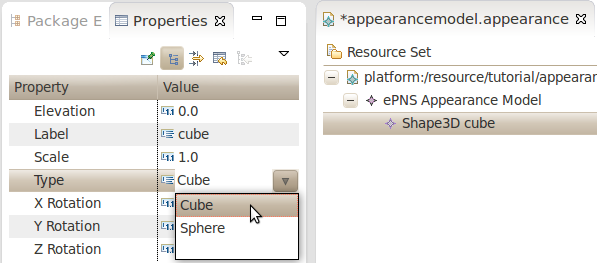
\includegraphics[width=12.0cm]{image/tutorial/Tutorial_10.png}
  \caption{Creation of a cube shape}
  \label{fig:tut10}
\end{center}
\end{figure}

\begin{figure}[htp]
\begin{center}
  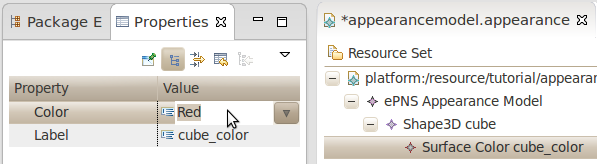
\includegraphics[width=12.0cm]{image/tutorial/Tutorial_11.png}
  \caption{Assigning an color to a shape}
  \label{fig:tut11}
\end{center}
\end{figure}

\begin{figure}[htp]
\begin{center}
  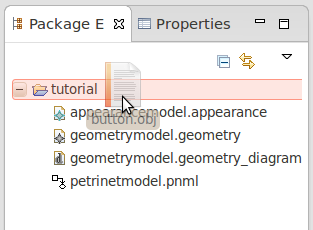
\includegraphics[width=6.0cm]{image/tutorial/Tutorial_12.png}
  \caption{Dragging and dropping a model file to the project folder}
  \label{fig:tut12}
\end{center}
\end{figure}

\begin{figure}[htp]
\begin{center}
  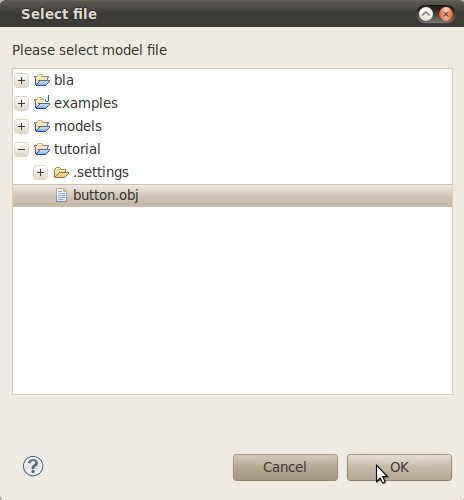
\includegraphics[width=8.0cm]{image/tutorial/Tutorial_13.png}
  \caption{Selecting a model file for the Model3D}
  \label{fig:tut13}
\end{center}
\end{figure}

\begin{figure}[htp]
\begin{center}
  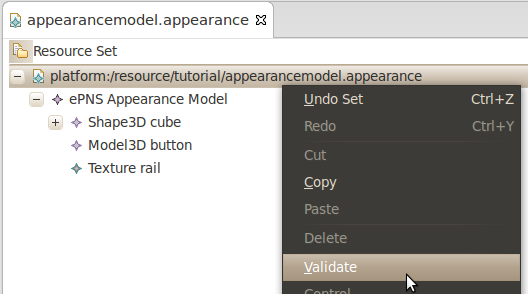
\includegraphics[width=10.0cm]{image/tutorial/Tutorial_14.png}
  \caption{Validating Appearance Model}
  \label{fig:tut14}
\end{center}
\end{figure}

\newpage
Now that all the necessary Appearances are created, you need to connect them to the corresponding elements. The appearance of the Tokens are
specified in the Petri net Model; the remaining Appearances (what Tracks and SimplePositions look like) should be set in the Geometry Model.
\begin{enumerate}
  \item To specify that the Token should look like a cube, you need to go back to the Petri net graphical editor. Edit the Label of the Token you created in the ordinary Place, assigning the name of the previously created shape ("cube") (See Figure \ref{fig:tut15}).
  \item To set the shape of the button, go to the Geometry graphical editor and modify the Appearance attribute of the Simple Position you
  created before (the one with the name "point"). Assign the same name as the corresponding Appearance ("button"). (See Figure \ref{fig:tut16}).
  \item To set the Appearance of the Track, modify the Appearance attribute of the Track "circle" to assign the same name of the
  Appearance ("rail").
\end{enumerate}

\begin{figure}[htp]
\begin{center}
  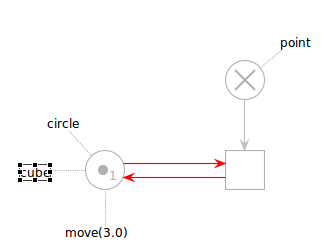
\includegraphics[width=6.0cm]{image/tutorial/Tutorial_15.png}
  \caption{Assigning "cube" appearance to the token}
  \label{fig:tut15}
\end{center}
\end{figure}

\begin{figure}[htp]
\begin{center}
  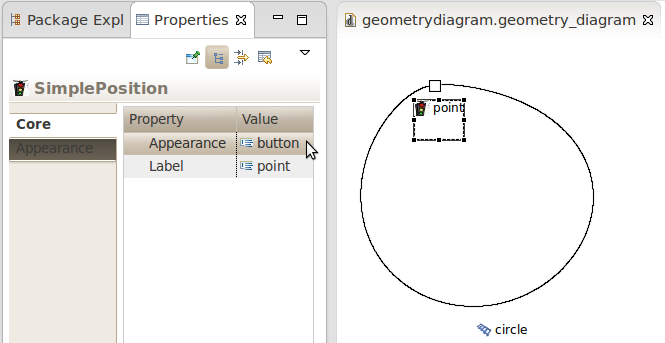
\includegraphics[width=12.0cm]{image/tutorial/Tutorial_16.png}
  \caption{Assigning "button" appearance to the simple position}
  \label{fig:tut16}
\end{center}
\end{figure}

\index{editors!validation}
The models are finished now. You have already checked that the Appearance Model have no errors, but you have to do the same with the 
Geometry and the Petri net Models (right click on the root node of the tree editor and click "Validate"). You will get an error in the 
Petri net Model because the IDs of the Petri net and the Page are not set. Modify them in the Properties View, and validate again. 
This time the validation will success.

Once you have configured the models and the simulation behaviour, you need to connect all the models using the Configurator. \index{configuration}
\begin{enumerate}
  \item Select again the project you created before in the Project Explorer and right click on it to select "New > Other > ePNS > 
  Configurator Model". Click "Next".
  \item Once again, the project you created should be selected as the parent folder (if it is not, change it). Give your Configurator 
  Model a name (keeping the \textit{.configurator} extension). Click "Finish".
  \item Open the file and right click the root node of the tree editor. Select "Load Resource...".
  \item A new window will appear where you can select the files you want to connect (See Figure \ref{fig:tut17}). Click "Browse Workspace...", 
  look for the project you are working in and select the \textit{.pnml} file you created before. Click OK twice to confirm your choice.
  \item Repeat the previous step to add the \textit{.geometry} and \textit{.appearance} files. 
  \item Once you have loaded the three files as resources, you need to attach them to the Configurator. To do this, open the Properties
  View of the Configurator object and edit its three properties selecting the corresponding model (in our case, "ePNS Appearance Model" 
  for ePNS Appearance, "ePNS Geometry" for ePNS Geometry and "Petri Net Doc" for ePNS Petri net) (See Figure \ref{fig:tut18}).
  \item Finally, you can set a default track width for the visualization. Modify the attribute of the Properties View and write "5.0".
\end{enumerate}

\begin{figure}[htp]
\begin{center}
  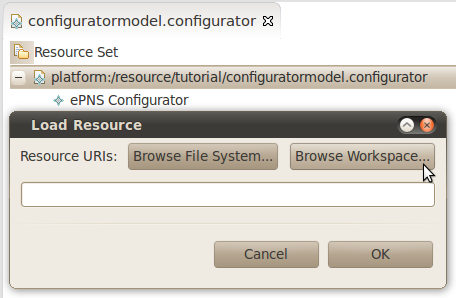
\includegraphics[width=7.0cm]{image/tutorial/Tutorial_17.png}
  \caption{Loading resources}
  \label{fig:tut17}
\end{center}
\end{figure}

\begin{figure}[htp]
\begin{center}
  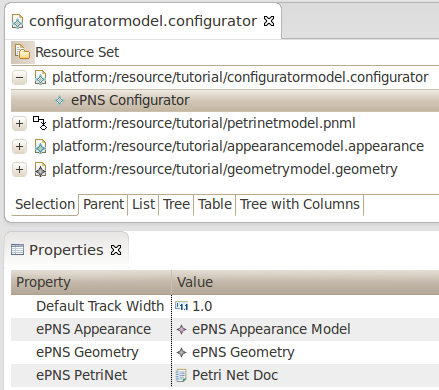
\includegraphics[width=10.0cm]{image/tutorial/Tutorial_18.png}
  \caption{Configurator properties}
  \label{fig:tut18}
\end{center}
\end{figure}

\newpage
By this point, the simulation is ready to be visualized. To start it you must right click on the Configurator object and select 
"Start simulator". \index{simulation}

After starting the Simulator, a new window like the one shown in Figures \ref{fig:tut19} and \ref{fig:tut20} will be displayed. 
Interacting with the simulation can be done in the following steps:
\index{simulation} \index{simulator}
\begin{enumerate}
  \item To start the Graphical Simulation animations, press the Start Button on the left side of the window. 
  \item In order to stop or pause the animation at any point, use the Stop/Pause/Resume\footnote{Please note that Resume is only available 
  after Pause has been clicked, and Stop is only available after Start has been clicked.} buttons available on the top of the window.
  \item Adding a new token in the place set us Interactive Input can be done by just clicking on its representation.
\end{enumerate}

\begin{figure}[htp]
\begin{center}
  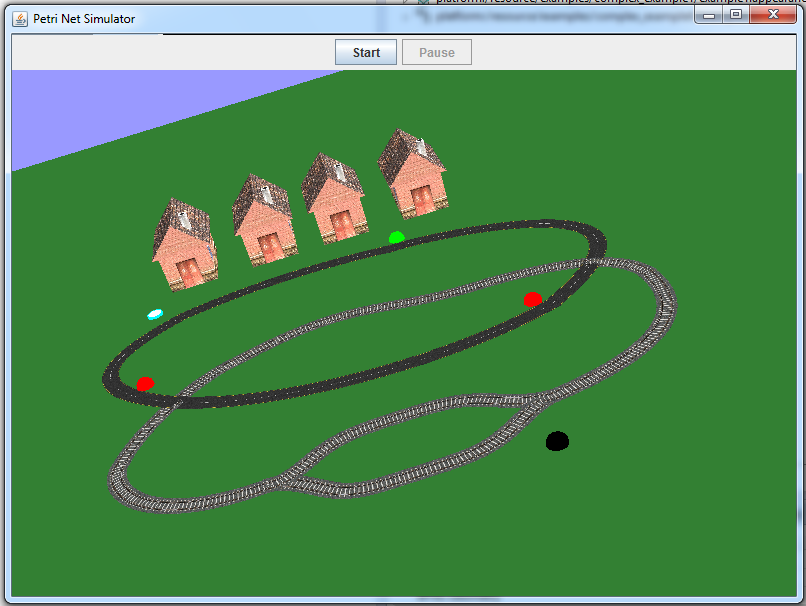
\includegraphics[width=10.0cm]{image/tutorial/Tutorial_19.png}
  \caption{Simulator interface - Before starting}
  \label{fig:tut19}
\end{center}
\end{figure}

\begin{figure}[htp]
\begin{center}
  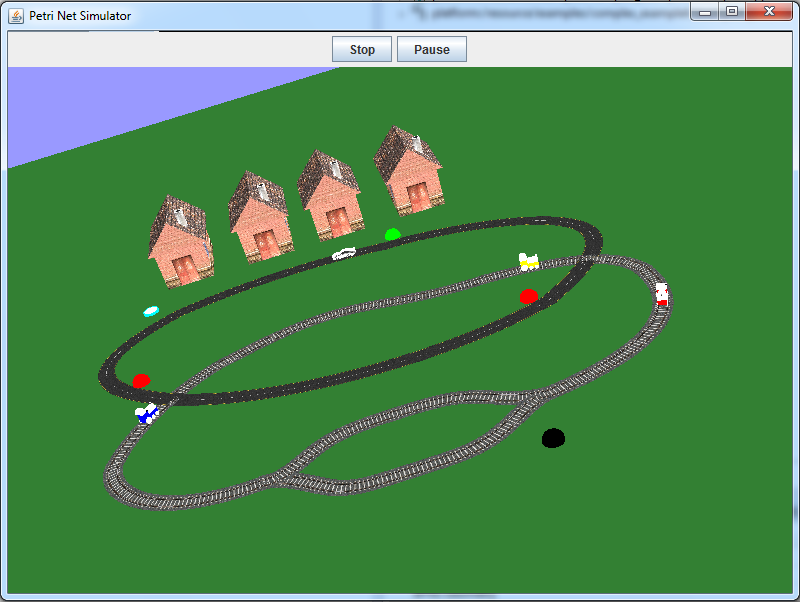
\includegraphics[width=10.0cm]{image/tutorial/Tutorial_20.png}
  \caption{Simulator interface - Simulation running}
  \label{fig:tut20}
\end{center}
\end{figure}


\section{User guide}
\label{sec:userguide}

\subsection{Before starting}
First, to create a ePNS file, the Eclipse runtime workbench should already be started. In it, the user should create an empty project so that it is later possible to group together all related files (PNML document, Geometry file, etc). An empty project can be created by selecting "File > New > Project > General > Project". Once this is done, there should be an empty folder in the Project explorer view.

\subsection{Petri net editor}
\index{ePNS Petri net}
\index{editors!Petri net}
\label{sec:userguide:petrinet}
\writer{Juan}

\subsubsection{Creating a new ePNS Petri net}
\label{sec:userguide:petrinet:create}
\index{ePNS Petri net!creation}
The creation of a Petri net file in an Eclipse runtime workbench will be detailed in this section. In this file the user will create the Petri net he/she would like to simulate and visualize.

Once the project has been created, the user can create a new Petri net file. To do so, he must right click on the project folder in the Project explorer view and select "New > Other > ePNK > PNML Document" \index{PNML Document} or do this via the "File" menu. The file creation wizard should have opened in a new window in Eclipse where a parent folder and a name for the Petri net file can be selected. The parent folder for the file can be chosen from the existing folders in the Eclipse environment (it is here one can select the empty project previously created to start grouping together all the files for the simulation). Any name can be given to the file as long as the \textit{.pnml} extension is kept. Once these two options have been adjusted, the file can be created by clicking on the "Finish" button.

Now that the file is created, some initial changes should be made in order to allow the edition of the Petri net. First, an ePNS Petri net document has to be created in the file. To do this, the recently created .pnml file should be opened and a child should be added to the "Petri Net Doc" by selecting the "New Child > Petri net (ePNS Petri net)" option in its right-click pop-up menu. \index{ePNS Petri net} Once the ePNS Petri net is created, a page should be added to it as a child by right clicking on it ("PetriNet") and selecting "New Child > Page".

\index{editors!validation}
One can now begin the edition of the Petri net (as described in the following sections). Once the editing process is completed, the Petri net has to be validated to check any errors that may have come up during said edition (e.g. conflicts with Arc Identies). This can be done by right-clicking on  the root element in the tree editor and selecting the "Validate" option.

\subsubsection{Adding items to the Petri net: Places, Transitions, Arcs, Tokens}
\label{sec:userguide:petrinet:add}
\index{ePNS Petri net!elements}
This section describes the addition of elements to a Petri net page previously created (see \ref{sec:userguide:petrinet:create}). These elements are the ones that describe the Petri net and it is from them that the simulation is inferred. This whole creation process can be done through a graphical editor that is shown by double clicking on the previously created page (see \ref{sec:userguide:petrinet:create}).

Three types of elements (nodes, arcs and labels, where tokens are a specific case of the latter) can be added to the Petri net, each of them in a different way.
\begin{itemize}
\index{ePNS Petri net!elements!node} \index{ePNS Petri net!elements!place} \index{ePNS Petri net!elements!transition}
\item The nodes of the Petri net can be either places or transitions, but they are all inserted in the same way. In the graphical editor the desired component must be selected by clicking on its corresponding icon in the \textit{Palette} shown on the right-hand side of the screen. After this, clicking on the canvas will insert a component of the selected type.
\index{ePNS Petri net!elements!arc}
\item The arcs of the Petri net connect nodes in the Petri net\footnote{Please note that arcs can only connect two different types of nodes between them.}. This can be done in the graphical editor there is an icon for arcs in the aforementioned Palette. Selecting it will enable the user to input arcs, which can be done by clicking on a node (this will be the arc's source 
\index{ePNS Petri net!elements!arc!source}) and dragging the mouse over to another node (this will be the arc's target 
\index{ePNS Petri net!elements!arc!target}).
\index{ePNS Petri net!elements!token}
\item The tokens of the Petri net are added to the places that have been previously created. The graphical editor presents the tokens as labels: to add a token to a place, create a label on the canvas (this can be done by clicking on the Label icon in the \textit{Palette} and clicking on the canvas) and link it to the place as a token (linking can be done by clicking on the outbound arrow that the label presents will selected and dragging it on to the place or by clicking on the Link Label icon in the \textit{Palette} and clicking on the label and the place; the label will represent a token if the \textit{Token} option is selected in the pop-up menu that appears when linking the label to the place).
\end{itemize}

\subsubsection{Setting some characteristics}
\label{sec:userguide:petrinet:setup}
\index{ePNS Petri net!attributes}
Once the components of the desired Petri net have been added to the page, some editing is in order
to customize it. This editing is done through the Properties view (shown when clicking on an element
and selecting the "Show Properties View" in its right-click pop-up menu) or through the graphical
editor, depending on the charasteristic to set. The different attributes that can be changed for
each element shall now be described:
\index{ePNS Petri net!attributes!Interactive Input} \index{ePNS Petri net!attributes!Geometry Label} \index{ePNS Petri net!attributes!Animations}
\begin{description}
\label{sec:userguide:petrinet:setup:places}
  \item[Places] have main four attributes that can be modified: \textit{Id},
  \textit{interactiveInput}, \textit{Geometry Label} and \textit{Animation Label}. The Id is used to
  identify the place; interactiveInput indicates if the place is an inputPlace, \index{input place}
  i.e. a place into which tokens can be inserted from the simulation, through a mouse click; the
  Geometry Label is used to associate the place with a geometry element (See
  \ref{sec:userguide:geometry:elements}); and the Animations label contains the animations
  associated to the place (See \ref{sec:userguide:animations}). The Id and interactiveInput feature
  can be edited in the Properties View by selecting each one and modifying its value (either writing
  on the text box or selecting from the options provided, depending on each attribute). The Geometry
  and Animations Labels must be added through the graphical editor by selecting a \textit{Label} in
  the Palette and clicking on the canvas. To associate it to a specific place, the user can either
  click on the label and drag the outgoing arrow that will appear over to the place, or click on the
  Link Label icon in the \textit{Palette} and click then on the label and the place. When releasing
  the click button, the \textit{Geometry Label} or \textit{Animation Label} option should be
  selected from the pop-up menu that is shown. The text in the label can be edited by selecting the
  label and writing the desired animation (See section \ref{sec:userguide:animations:types}).
  Besides, if the place is an Input Place, a fifth attribute can be added: Input Place Appearance
  Label, a Label that indicates the appearance of the tokens externally inserted in that place. This
  label is created in the same way as Geometry or Animation Labels.
 \item[Tokens in Places] can have an \textit{appearance} associated to them, which indicates their
 graphical representation in the simulation. This characteristic is set by editing the text of the
 Token Label (this text can be anything, although later it must coincide with the name of an
 appearance created in the Appearance Editor; for more information see
 \ref{sec:userguide:appearance}).
 
 \item[Transitions] have the attribute \textit{Id}, which can be modified in the Properties View.
 \label{sec:userguide:petrinet:token:appearance} \index{ePNS Petri net!attributes!Appearance}  
  
\index{ePNS Petri net!attributes!identity}
  \item[Arcs] have one attribute, \textit{identity}, which can be edited through the Properties View. It is used to determine the trajectory of the tokens when a 
  transition is fired.
\end{description}

\subsubsection{Animations}
\index{animations}
\label{sec:userguide:animations}
Introducing animations into a Petri net model will allow the user to define the way in which the behaviour of the Petri net is represented in the final graphical visualization. The animations will be applied to Tokens when they move into a Place, so it will be in these last elements where Animations shall be edited. This is done by writing on an \textit{Animation Label} in the Petri net editor (see \ref{sec:userguide:petrinet:setup:places} for more details). Here the different types of Animations and their parameters shall be described, as well as the syntax that must be used to properly insert them into the Petri net. 
\index{animations!move}

\label{sec:userguide:animations:types}
The animations that can be used for the visual representation of a Petri net are the following:

\begin{description}
  \item[Move:] written as \textit{move(speed)}, this Animation will move graphical representation of the Token (see \ref{sec:userguide:petrinet:token:appearance}) at a certain \textit{speed} along the track assigned (as a Geometry Label) to the Place. \index{animations!move}
  \item[Wait:] written as \textit{wait(time)}, the 3D Engine managing the visualization will simply do nothing to the Token's representation for the specified amount of \textit{time} (in miliseconds). \index{animations!wait}
  \item[Show:] written as \textit{show(label)}, it shows the object referenced by the \textit{label} (see \ref{sec:userguide:appearance} in the position of the 2D plane connected (as a Geometry Label) to the Place.
  \item[Hide:] written as \textit{hide()}, it hides from view the object that is in the position of the 2D plane connected (as a Geometry Label) to the Place. \index{animations!hide}
  \item[Sequence:] this is a special type of Animation composed of two or more of the previously described Animations. It must be written following the scheme \textit{animation;animation;...}, i.e., as animations separated by semicolons. \index{animations!sequence}
\end{description}

%%%%%%%%%% Geometry Editor %%%%%%%%%%%
\subsection{Geometry Editor}
\writer{George, Jerome}
\index{geometry}
\index{editors!geometry}
\label{sec:userguide:geometry}

%%% New geometry file
\subsubsection{Creating a new Geometry file}
\label{sec:userguide:geometry:create}
This section will explain how a Geometry file can be created using the Eclipse runtime workbench.

A Geometry file can be created with the use of wizards. Like all Eclipse creation wizards, the one
that is needed for Geometry file creation can be accessed via the \textit{New} menu, either by
clicking on the "File" menu of the menu bar or by right-clicking on the Explorer of the workbench.
The user then has to choose "Other..." for moving to the next "Select a wizard" dialog. What has
been done so far could be also achieved by pressing "Ctrl+N", a shortcut that makes things simpler.
Now, the user is ready to finally choose the type of file he wants to create. In the "Select a
wizard" dialog he can either type the string "Geometry Diagram" - note that is not case sensitive -
or he can find this option under "Examples", in the same dialog.

In the dialog "Create Geometry Diagram" the user can change the name given to the graphical editor. In the last step, by selecting "Next" he can optionally change the name of the tree editor as well. This task is completed by clicking on "Finish". Now the user should be able to see the new project place in the runtime workbench Explorer.

%%% General stuff about geometry elements
\subsubsection{Geometry elements: TrackPosition, Track, SimplePosition}
\label{sec:userguide:geometry:elements}
\index{geometry!track} \index{geometry!simple position} \index{geometry!track position}
There are two editors with which the user can create a Geometry, the tree editor and the graphical editor. Nevertheless we will see later that the graphical editor is safer and easier to use, so the tree editor shouln't be used in most of the cases. These editors can be populated with some elements, namely \textit{Tracks}, \textit{TrackPosition} and \textit{SimplePosition}. 

A \textbf{Track} represents the path that a track-bound object will move on. A \textbf{TrackPosition} denotes either the starting point of a Track or its ending point. As as far as the Track element is concerned, it should be linked with two TrackPosition so that the Geometry is valid. The two following sections (\ref{sec:userguide:geometry:tree} and \ref{sec:userguide:geometry:graphical}) will explain how to add such objects, describing the editors in details. Last but not least, a \textbf{SimplePosition} represents a point on the Geometry of a particular interest. On this point a static object, a traffic light for instance, can be put to control the behavior of the track bound moving object that follows the path that a Track elements has defined. A SimplePosition can be placed anywhere in the Geometry. 

%%% Howto use the tree editor
\subsubsection{The tree editor}
\label{sec:userguide:geometry:tree}
The tree editor is the one of the two editors that becomes available after the creation of a new Geometry file. The file-format for this editor is recognized by the ".geometry" suffix. Double-clicking on a file of that type will start the tree editor. The user can also edit this type of file by clicking on the little arrow on the left of the filename ending with a ".geometry" while he is inside the Explorer. With this editor the user can create and delete elements of the Geometry. However it is advisable to use the graphical editor for that purpose instead, since it is easier to use and the user gets an immediate picture of the changes he/she is doing to the Geometry. Indeed, the use of the graphical editor for creation and deletion of Geometry elements is safer, since inconsistencies might emerge otherwise between the two editors. This is the reason why this document does not elaborate more on how to create or delete Geometry elements in the tree editor. Figure \ref{fig:geo_tree_editor} shows an overview of the tree editor editing a Geometry file.

\begin{figure}[htp]
\begin{center}
  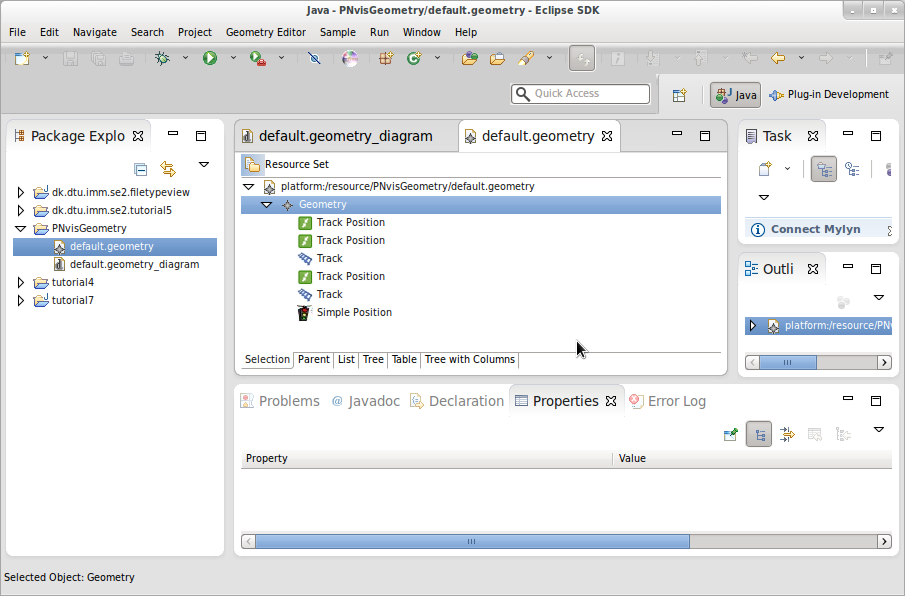
\includegraphics[width=10.0cm]{image/geo_tree_editor.png}
  \caption{Overview of the tree editor for a Geometry file}
  \label{fig:geo_tree_editor}
\end{center}
\end{figure}

\index{editors!validation}
An important action that the user can perform using the tree editor is to validate the Geometry he has built. This can be done by right-clicking on the top element of the tree editor. Then, in the pop-up menu he has to select "Validate". If the validation succeeds the user will be notified with a message on the emerged dialog. In case of validation failure the same dialog will give the user the user the chance to investigate failure related messages by clicking on the "Details" button. 

%%% Howto use the graphical editor
\subsubsection{The graphical editor}
\label{sec:userguide:geometry:graphical}
The graphical editor is the second editor that becomes available after the creation of a new Geometry file. It should be used to edit these Geometry files as it is safer and easier to use than the tree editor. The file-format for this second editor can be found thanks to the ".geometry\_diagram" suffix. To open this editor the easiest way is to double-click on a file with that suffix and that previously created inside the Explorer (see section \ref{sec:userguide:geometry:create}). Figure \ref{fig:geometry_overview} shows an overview of the graphical editor with an open Geometry file.

\begin{figure}[htp]
\begin{center}
  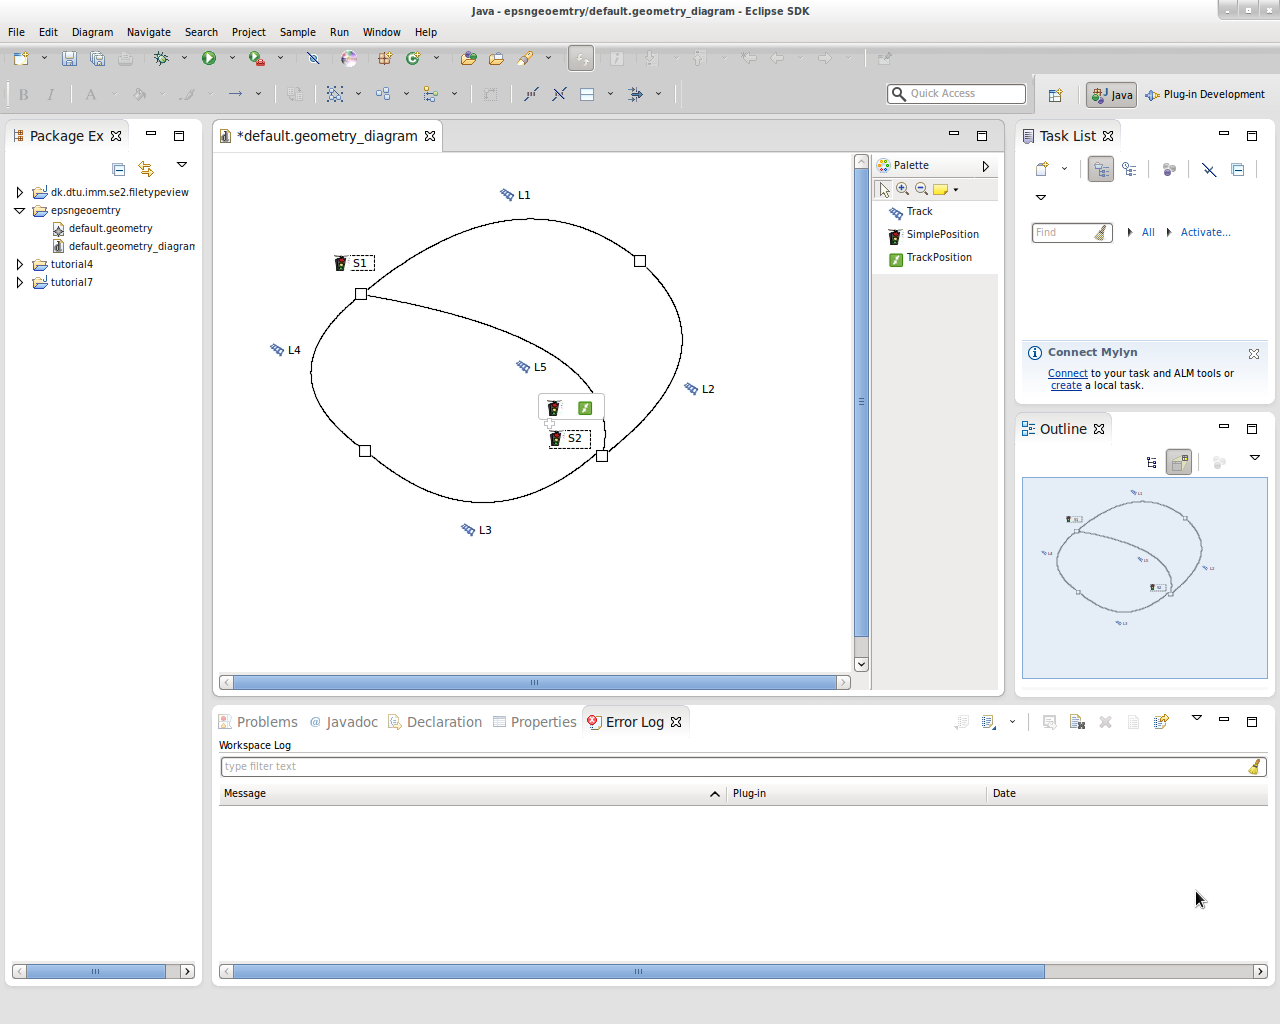
\includegraphics[width=10.0cm]{image/geometry_general.png}
  \caption{Overview of the graphical editor for a Geometry file}
  \label{fig:geometry_overview}
\end{center}
\end{figure}

On the right-side of the editor, the \textit{palette} or tool bar of the graphical editor can be seen. This allows the user to create Geometry objects. We will come to that part a little bit later. At the top, the \textit{tab} of this page can also be seen, displaying the name of the document. 

To create Geometry objects the user needs to click on the element he wants to create inside the \textit{palette} and drop it where he wants it to be inside the canvas. There are three different objects he can create with the graphical editor for Geometry files : a TrackPosition, a Track, and a SimplePosition. He can have a look at section \ref{sec:userguide:geometry:elements} to understand in which case each element should be used. It must be noted that the reader cannot create a Track if he/she has not previously created at least one TrackPositions. 

%Finally the user can undo and redo actions by using the shortcuts "CTRL+Z" (undo) or "CTRL+SHIFT+Z" (redo) or by clicking on the corresponding entries in the "Edit" menu. Indeed the user can save his document by hitting "CTRL+S" or "File" -> "Save".% // Ekkart said : useless...

%%% Set characteristics
\subsubsection{Setting some characteristics}
\label{sec:userguide:geometry:characteristics}
Ultimetaly, the reader must set some characteristics of the Geometry objects in order to make the simulation running with appropriate visuals. These characteristics can be inspected at the Properties View  for each object. If this view is not visible in the workbench, go to the menu "Windows" -> "Show View" -> "Other..." and inside "General" double-click on the "Properties" (view). This view will now display additional properties for each object selected. Some of this properties are already defined, such as the starting point and ending point of a Track, while others need to be defined, for instance the AppearanceLabel of a Track.

\label{sec:userguide:geometry:appearance}
To configure correctly the Geometry file the user must define some of these additional properties. For the Track object and the SimplePosition object the user will have to define an AppearanceLabel that is a label refering to some appearance defined in the Appearance Editor (see section \ref{sec:userguide:appearance:new}). This can be done by clicking on the object once created and double-clicking in the right-zone corresponding to the AppearanceLabel inside the properties view, then writing some text using the keyboard. For the TrackPosition object the user will not have to define anything more.

Finally, the user can change the Label of some Tracks and SimplePositions by clicking on the name-label inside the graphical editor and start typing the new name or by selecting the object and changing the value of the field Label inside the properties view.
%%%%%%%%%%%%%%%%%%%%%%%%%%%%%%%%%%%%%

\subsection{Appearance Editor}
\index{appearance}
\index{editors!appearance}
\label{sec:userguide:appearance}
\writer{Pablo}

\subsubsection{Creating a new Appearance file}
\label{sec:userguide:appearance:create}
The creation of an Appearance file is done by selecting "New > Other > Example EMF Model Creation Wizards > Appearance Model" and clicking on the "Next" button. The next window allows both the selection the parent folder for the file and the edition of the name of said file (maintaining the \textit{.appearance} extension). After editing these two things and clicking on the "Next" button, the option "ePNS Appearance Model" must be chosen as a Model Object. Clicking on "Finish" will create the Appearance file.

\subsubsection{Adding items to the Appearance: Model3D, Shape3D, Texture, SurfaceColor}
\index{appearance!Model3D} \index{appearance!Shape3D} \index{appearance!Texture} \index{appearance!SurfaceColor}
\label{sec:userguide:appearance:add}
Once there is an Appearance file created (see above), elements can be added to it. To do it the Appearance file must be open and its root node expanded. In said node will be a node "ePNS Appearance Model", where right clicking permits the addition of an element to the Appearance file by means of the "New Child" option. Here the user can choose between four elements: Model3D, Shape3D, Texture and SurfaceColor.
\subsubsection{Setting some characteristics}
\index{appearance!attributes}
\label{sec:userguide:appearance:edit}
Simply having an Appearance file created and adding elements to it will not suffice, for these elements need to refer to something that describes the Appearance, as well as having a name to associate them to the components of the Petri net. The attributes of each element that can be edited are here presented, each of them editable in the Properties view of the selected element:
\index{appearance!Model3D} \index{appearance!Shape3D} \index{appearance!Texture} \index{appearance!SurfaceColor}
\begin{itemize}
  \item All elements have a \textit{label} attribute that gives each one a name and will later allow the connection to the components of the Petri net.
  \item Both \textbf{Model3D} and \textbf{Shape3D} objects have: a \textit{scale} to make them bigger or smaller; three rotation values (\textit{xRotation}, \textit{yRotation} and \textit{zRotation}) to rotate them; and an \textit{elevation} attribute to raise the shape.
  \item \textbf{Model3D} also has a \textit{file} attribute, which is a reference to a file where the desired Appearance is described. This file must be located in the Ecplipse workbench.
  \item A \textbf{Shape3D} also allows the modification of its \textit{type} attribute. This attribute grants the user the choice to select the object's Appearance among a series of predefined shapes (cube, sphere...).
  \item A \textbf{Texture} has a \textit{file} attribute analogous to the \textit{file} attribute in the Model3D (again, this file must be located in the Ecplipse workbench).
  \item Finally, the \textbf{SurfaceColor} will have a \textit{Color}, which can be chosen from the 13 predefined colours.
\end{itemize}

Shapes (Model3D and Shape3D elements) can also have a surface (Texture or SurfaceColor). To add this, right-click on the desired shape and select "New Child" and "Texture" or "SurfaceColor". The properties of the selected surface can be changed again using the Properties View.

\subsubsection{Adding appearances to Tokens, Tracks and Simple Positions}
To add appearances to Tokens, Tracks and SimplePositions, one must have created both a Petri net and a corresponing Geometry. See \ref{sec:userguide:geometry:appearance} and \ref{sec:userguide:petrinet:token:appearance} for information on how to do this.

\subsection{Configuration Editor}
\label{sec:userguide:configuration}
\index{configuration}
\index{editors!configuration}
\writer{Marius}

\subsubsection{Creating a new Configuration file}
\label{sec:userguide:configuration:new}
This subsection gives details on the creation and proper setting of a Configuration file.
With all the Geometry, Appearance and PNML resources created, a Configuration file is needed, to link them all together. The Configurator gives the user the possibility to use, for example, the same Geometry and PNML files, but with a different Appearance file.
To create a new Configurator file, the user must go to File -> New -> Other, and from Example EMF Model Creation Wizards select Configurator model and click Next. From there, he should select a parent folder, give the new file a name and click on Finish. 

\subsubsection{Loading resources and setting Configurator properties}
To load the resources and set the Configurator properties, the user should first open the Configurator file. In the tree-view, it can be seen that the file contains a Configurator object. Here, the Appearance, Geometry and PNML resources need to be loaded. This is done by right-clicking in the active window and selecting "Load Resource". Then, after having selected "Browse Workspace", the Appearance file created as in step \ref{sec:userguide:configuration:new} must be selected and click Ok. The same process must be repeated for the Geometry and PNML files. The order in which these files are loaded is not important. They can also be loaded all at once. 

To set the configurator properties, the user has to click on the Configurator and in the property view, in the Appearance field, he should click on the Value field and select "ePNS Appearance Model" from the dropdown menu. Similarly, for the Geometry property, "epns.geometry" must be loaded, and for Petri net, "Petri Net Doc" must be selected. Another property that the user should set is the Default Track Width. Its default value is 1.0, but a bigger value is recommended, so that the tracks can be easily distinguished.

\subsubsection{Starting a simulation}
With the Geometry, Appearance and PNML resources loaded and selected in the configurator, to start
the simulator, the user has to right-click on the Configurator object and select the \textit{Start
simulator} menu item. A new window will appear, in which the simulation would run. More details can
be found in section \ref{sec:userguide:simulator}.

\subsection{Simulator}
\label{sec:userguide:simulator}
\index{simulator}
\writer{Ruxandra}

\subsubsection{Starting the simulator}

The Simulator can be started by clicking on the Start Simulator option after right clicking on the Configuration 
item from the .configurator file, after loading and linking the geometry, the appearance and the Petri net files, 
as described in \ref{sec:userguide:configuration}.

\subsubsection{Controlling the simulation: Play/pause/stop}
After starting the simulator, a new window like the one shown in figure \ref{fig:simulator} will be displayed.
The simulation can be played by pressing the Start Button on the left side of the window. 

The simulation can be stopped at any time. By stopping it, the simulation will return to the initial state. The 
simulation can then be played again by pressing the Start button.

At any time, the simulation can be paused, by pressing the Pause button. It can then be resumed by pressing the Resume button, which will
replace the Pause button after a pause.

\begin{figure}[htp]
\begin{center}
  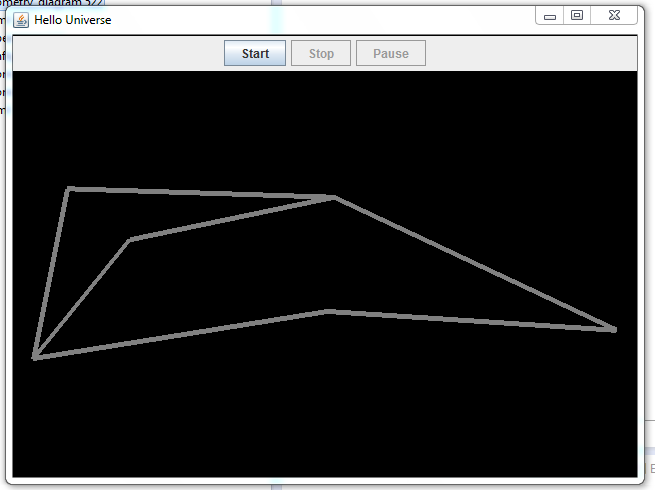
\includegraphics[width=10.0cm]{image/simulator.png}
  \caption{Simulator interface}
  \label{fig:simulator}
\end{center}
\end{figure}

\subsubsection{User Interaction}
\index{input place}
The user can interact with the animation by using the input places. The interactivity for a place is set in the 
pnml file as described in section \ref{sec:userguide:petrinet:setup}. If a place is an input place, it usually has associated
an appearance as a Single Object and is placed on a SimplePosition (see section \ref{sec:userguide:geometry:elements} for details) , rather than a track. 
In this way, the user can click on the object visually associated to the place and insert a token into the place.
Another way the user can interact with the simulation is by changing the view point. There are 3 ways to move that camera: scroll to zoom in/out,
right click and drag to pan the camera and left click and drag to rotate the camera.




\section{Glossary}
\writer{Georgios}

\subsection{Technical Glossary}
\begin{description}
  \item[Animation] The dynamic behavior of objects on 3D Canvas that are associated with Places of the Petri Net model.
  \item[Appearance] The look and feel of the objects visualized by the 3DEngine .
  \item[Appearance Editor] A graphical editor provided EMF for configuring appearance.
  \item[Control GUI] A simple Graphical User Interface with appropriate actions (play/pause/stop buttons) so as the end user to be able to interact with the 3DEngine and consequently with underlying Petri Net execution .
  \item[Geometry] the track (3D line/curve) on which the 3D-visualization of the Petri Net simulation takes place. The geometry consists of predefined objects such as, semicircles, points and lines.
  \item[Geometry Editor] A graphical editor provided by ePNK and GMF for designing the area on which the simulation will be reflected.
  \item[Identity] The attribute of Arcs in the Petri Net model that defines the trajectory of the Tokens.
  \item[IgnoreAnimation] The attribute of Arcs in the Petri Net model that allows the target transition to fire without the associated Place Animation having finished.
  \item[Input place] a place in which tokens can be insterted externally, i.e. by clicking an interactive control point.
  \item[Interactive control point] A point that allows the user to interact with the system (e.g. by a click)
  \item[Petri Net Editor] A graphical editor provided by ePNK and GMF for designing the Petri Net of the system a user wants to visualize.
  \item[Physical object] A graphical object that is used by the 3DEngine for visualizing its behaviour during the Petri Net simulation.
  \item[Simulator] The software component that will provide the underlying Petri Net execution information to the 3DEngine so as to be able to visualize the Petri Net execution with 3D objects.
  \item[Shape] The visual traits of a physical object being part of the simulated system visualization.
  \item[Token] The Petri Net element that moves along Petri Net places through transitions.
\end{description}

\subsection{Technology Terms}
\begin{description}
\item[Ecore Tool editor] - The EMF editor that provides all the necessary elements for realizing or drawing the model in question.
\item[EMF] - The Eclipse Modeling Framework. It auto-generates code that represents the corresponding model (usually described in UML).
\item[EMF Validation Framework OCL Integration] -  Helps for expressing constraints on ambiguous graphical models such as a class diagram. Tightly used with UML users can define constraints on their models.
\item[ePNK] - The eclipse Petri Net  Kernel, a modern equivalent of PNVis missing the visualization part though. Built following the model-based software engineering paradigm. ePNK Petri Net Types to be extended to provide new functionality.
\item[GMF] - The Eclipse Graphical Modeling Framework provides the appropriate infrastructure for developing graphical editors based on EMF.
\item[Xtext] - Xtext is a framework for development of programming languages and domain specific languages.
\end{description}

\printindex

\end{document}

